\newif\ifglobal

%%%%%%%%%%%%%%%%%%%%%%%
%%% Compile to view %%%
%%%%%%%%%%%%%%%%%%%%%%%

%%%%%%%%%%%%%%%%%%%%%%%%%%%%%%%%%%%%%%%%%%%%%%%%%%%
%%% Readme:                                     %%%
%%% https://www.overleaf.com/read/bwdjvfjksvjy/ %%%
%%%%%%%%%%%%%%%%%%%%%%%%%%%%%%%%%%%%%%%%%%%%%%%%%%%

% >>> M?: marks a module setting number or important notice

% >>> M4: Set {./relative-path} to external files for this module <<<
\def \modulefiles {./18-SDHOST}
% To add an external file, use:
% (Replace '---' with actual filename)
% '\input{\modulefiles/tables/---.tex}' for tables
% '\includegraphics{\modulefiles/figures/---}' for figures
% '\subfile{\modulefiles/---}' for register files

% >>> M1: This module is in global project? <<<
% 'YES' - uncomment; 'NO' - comment out
\globaltrue

\ifglobal
    \documentclass[main\_\_CN.tex]{subfiles}

\else
    % Font "FandolSong-Regular" used by ctex does not have GSUB table.
    % It causes warnings that do not affect compilation and can be ignored.
    \PassOptionsToPackage{quiet}{fontspec}

    \documentclass[openany, 10pt]{book}

    % >>> M2: In ./00-shared/preamble-trm-module, also find
    %         settings for visibility of todo notes, watermark <<<
    \usepackage{preamble-trm-module}


    % Enable Chinese typesetting
    \usepackage{ctex}

    % >>> M3: Temporary labels in Chinese
    %         you can add your own labels there <<<
    \myexternaldocument{./00-shared/temp-labels-cn}

\fi %\ifglobal


\setcounter{secnumdepth}{4}

% >>> M5: If this module needs any updates in
% './00-shared/preamble-trm-module.sty'
% (include additional package, etc.), contact your module PM
% or create the file './00-shared/changelog.tex' make the
% necessary updates yourself and document them in this file <<<


\begin{document}


% Sets language into which pre-defined bits of text are translated
\selectlanguage{chinese}

% Do not delete this block
\ifglobal
% Add the following front matter if
% this module is outside of global project
\else
    \InputIfFileExists{readme}{}{}
    {\let\clearpage\relax \listoftodos}
    \tableofcontents
    %\listoftables
    %\listoffigures
\fi


%%%%%%%%%%%%%%%%%%%%%%%%%
%%% TRM Module Begins %%%
%%%%%%%%%%%%%%%%%%%%%%%%%
\hypertarget{sdhost}{}
\chapter{SD/MMC 主机控制器 (SDHOST)}
\label{mod:sdhost}

\section{概述}

\chipname{} 存储卡接口控制器提供了一个访问安全数字输入输出卡 (SDIO)、MMC 卡和 CE-ATA 设备的硬件接口，用于连接高级外围设备总线 (APB) 和外部存储设备。该控制器支持两个外部卡（卡 0 和卡 1）。所有 SD/MMC 模块接口信号都须通过 GPIO 矩阵传输至 GPIO pad。

\section{主要特性}
该模块支持以下特性：

\begin{itemize}
\item 支持两个外部卡
\item 支持 3.0、3.01 版本 SD 存储卡标准
\item 支持 4.41、4.5、4.51 版本 MMC
\item 支持 1.1 版本 CE-ATA
\item 高达 80 MHz 的时钟输出
\item 支持 1-bit、4-bit 和 8-bit 位宽模式
\end{itemize}

\begin{tiplisting}
在 80 MHz 工作条件下，时钟相位调节能力受限，仅支持 0° 和 180° 两种相位配置。PCB 布局设计时应充分考虑该限制，以确保时序收敛。更多细节请参考 \ref{sec:sdhost-phase-selection} \textit{\nameref{sec:sdhost-phase-selection}} 小节。
\end{tiplisting}

SD/MMC 控制器连接的拓扑结构如图 \ref{fig:sdhost-card-sys-topo} 所示。该控制器支持两组外设工作，但不支持同时工作。

\begin{figure}[ht!]
    \centering
 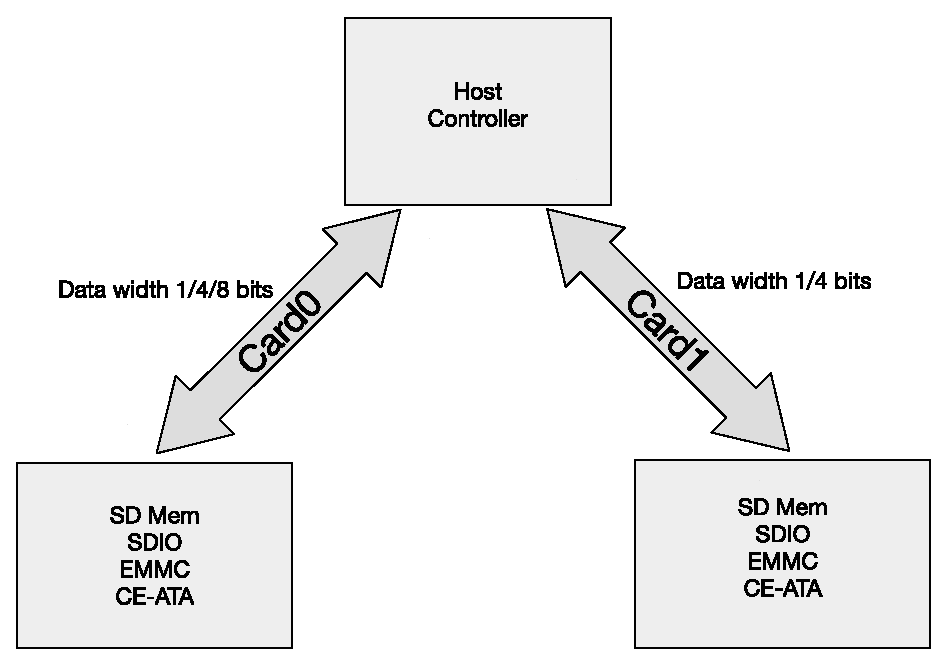
\includegraphics[width=0.55\textwidth]{./18-SDHOST/figures/18-SDHOST-card-system-topo}
    \caption{SD/MMC 控制器连接的拓扑结构}
    \label{fig:sdhost-card-sys-topo}
\end{figure}

\section{SD/MMC 外部接口信号}

SD/MMC 的外部接口信号主要为时钟信号 (sdhost\_cclk\_out\_1.eg:card1)、命令信号 (sdhost\_ccmd\_out\_1)、数据信号 (sdhost\_cdata\_in\_1[7:0]/sdhost\_cdata\_out\_1[7:0])，SD/MMC 控制器可通过这些外部接口信号与外部设备通信。其它信号还包括卡中断信号、卡检测信号和写保护信号等。各个信号的方向如图 \ref{fig:sdhost-ext-sign} 所示。每个管脚的方向和描述如表 \ref{tab:sdhost-signal-description} 所示。
\clearpage
\begin{figure}[ht!]
    \centering
    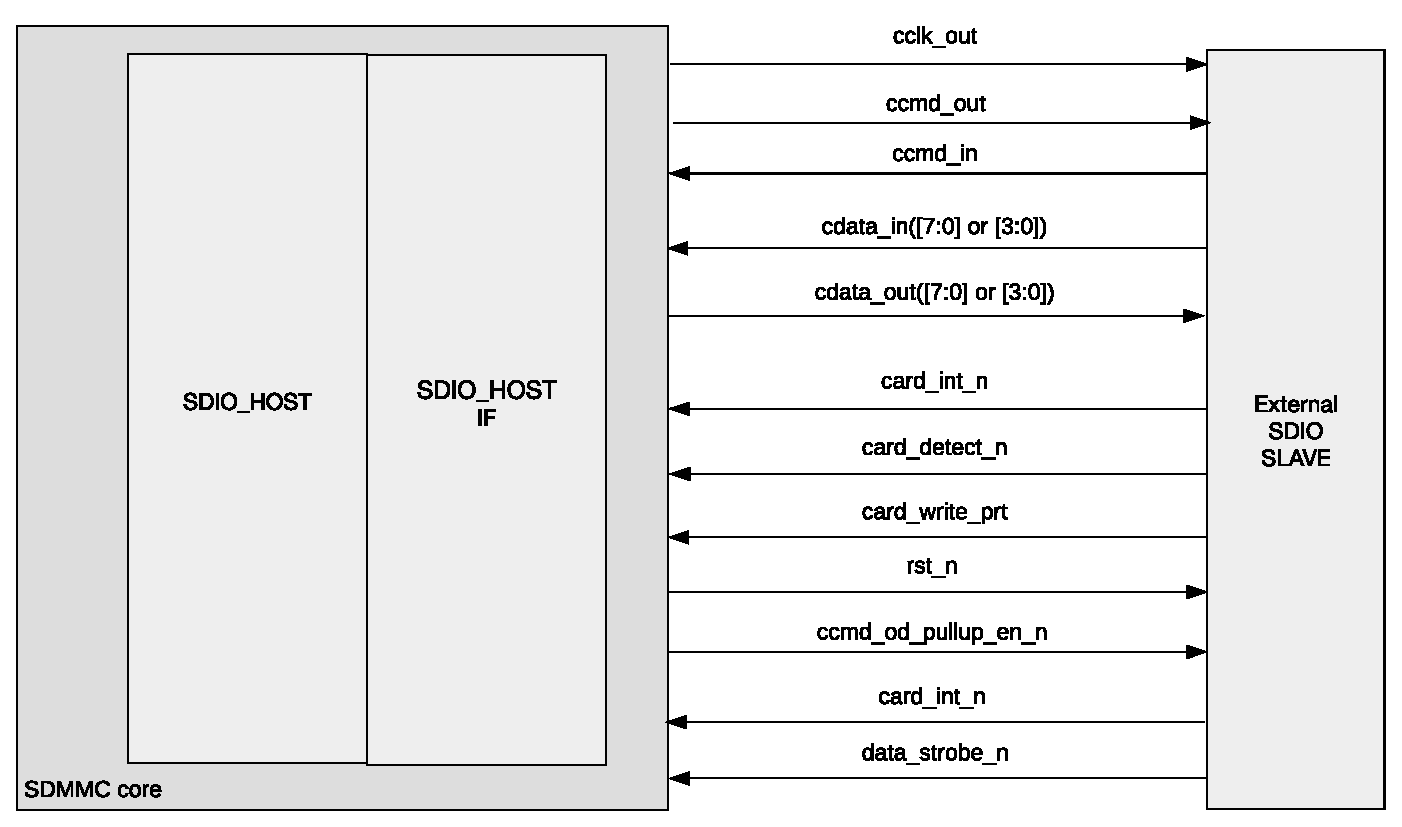
\includegraphics[width=0.6\textwidth]{./18-SDHOST/figures/18-SDHOST-external-signals}
    \caption{SD/MMC 控制器外部接口信号}
    \label{fig:sdhost-ext-sign}
\end{figure}

\input{./18-SDHOST/tables/18-SDHOST-signal-desc__CN}

\section{功能描述}
\subsection{SD/MMC 主机控制器结构}
SD/MMC 主机控制器主要由两大功能块组成，如图 \ref{fig:sdhost-block-diag} 所示，分别为：

\begin{itemize}
    \item 总线接口单元 (BIU)：提供 APB 总线访问寄存器的接口、RAM 数据访问方式 和 DMA 数据读写操作
    \item 卡接口单元 (CIU)：处理外部存储卡的接口协议，控制时钟。
\end{itemize}

\begin{figure}[ht!]
    \centering
    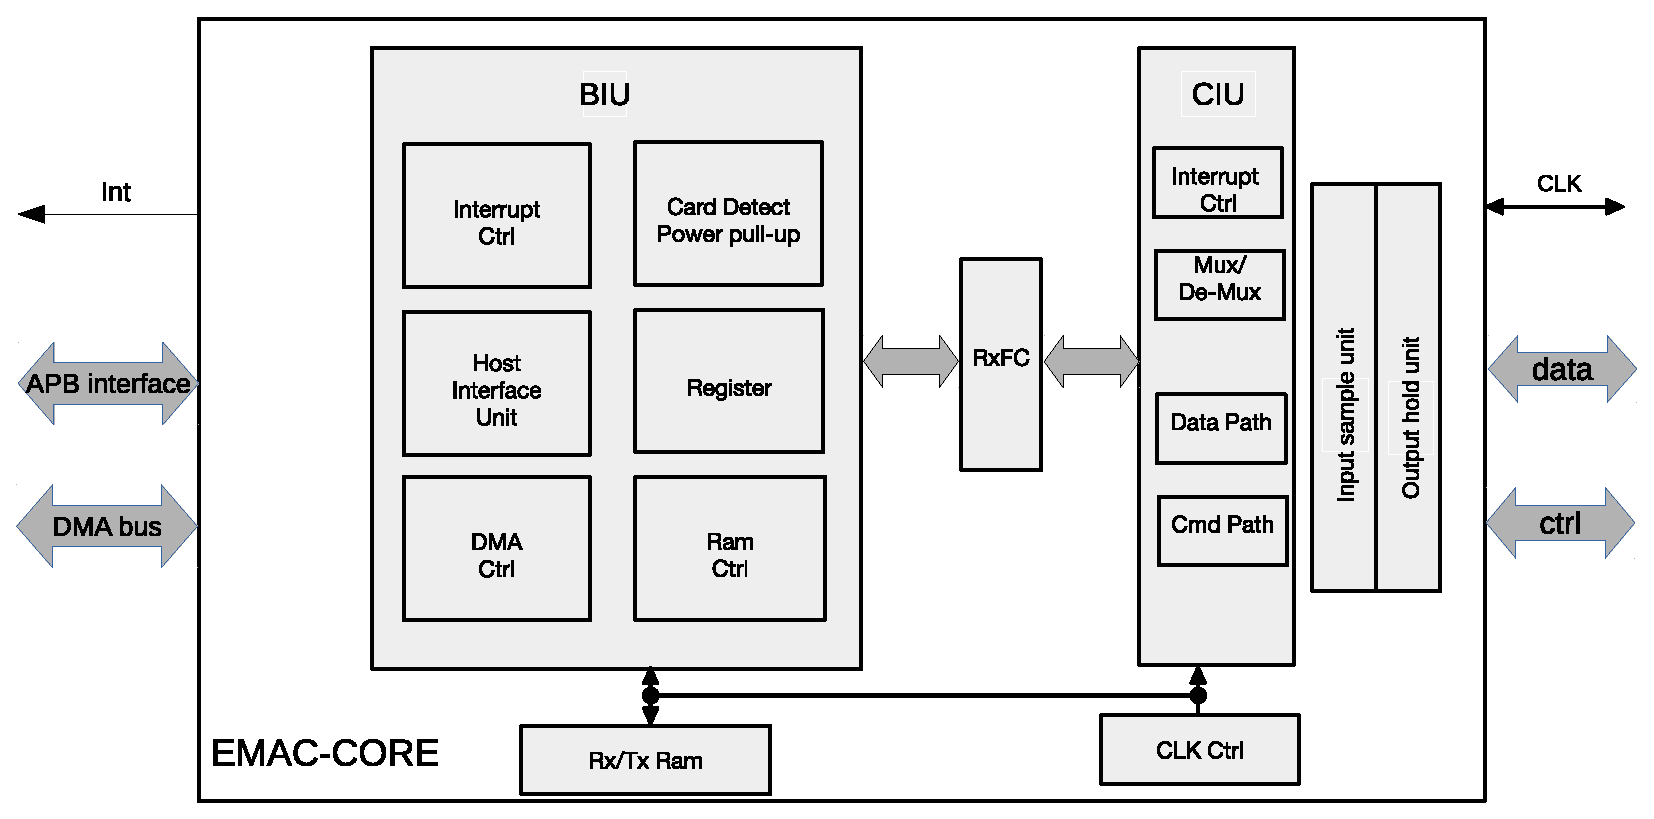
\includegraphics[width=0.8\textwidth]{./18-SDHOST/figures/18-SDHOST-block-diagram}
    \caption{SDIO 主机结构框图}
    \label{fig:sdhost-block-diag}
\end{figure}

\subsubsection{总线接口单元 (BIU)}
该模块提供了通过主机接口单元 (HIU) 访问寄存器和 RAM 数据的方式。除此之外，它通过 DMA 接口提供独立的 RAM 数据访问。它通过 DMA 接口访问 Memory 中的数据。图 \ref{fig:sdhost-block-diag} 描述了该模块的内部结构。图 \ref{fig:sdhost-clk-phase-selec} 描述了时钟相位选择。

BIU 支持以下功能：

\begin{itemize}
	\item 主机接口
	\item DMA 接口
	\item 中断控制
	\item 寄存器访问
	\item FIFO 访问
	\item 上电/上拉控制和卡检测
\end{itemize}

\subsubsection{卡接口单元 (CIU)}
该模块实现卡专用接口协议。在 CIU 中，命令通路 (Cmd Path) 控制单元和数据通路 (Data Path) 控制单元将控制器分别连接到 SD/MMC/CE-ATA 卡的命令接口和数据接口。CIU 还提供时钟控制。图 \ref{fig:sdhost-block-diag} 描述了 CIU 的内部结构。

CIU 由以下主要功能模块组成：

\begin{itemize}
	\item 命令通路
	\item 数据通路
	\item SDIO 中断控制
	\item 时钟控制
	\item Mux/De-Mux 单元
\end{itemize}

\subsection{命令通路}

命令通路具有以下功能：
\begin{itemize}
	\item 配置时钟参数
	\item 配置卡命令参数
	\item 向卡总线发送命令 (sdhost\_ccmd\_out)
	\item 从卡总线接收响应 (sdhost\_ccmd\_in)
	\item 向 BIU 发送响应
	\item 在命令线上发送 P-bit
\end{itemize}

命令通路状态机如图 \ref{fig:sdhost-cmd-state-machine} 所示。

\begin{figure}[ht!]
    \centering
    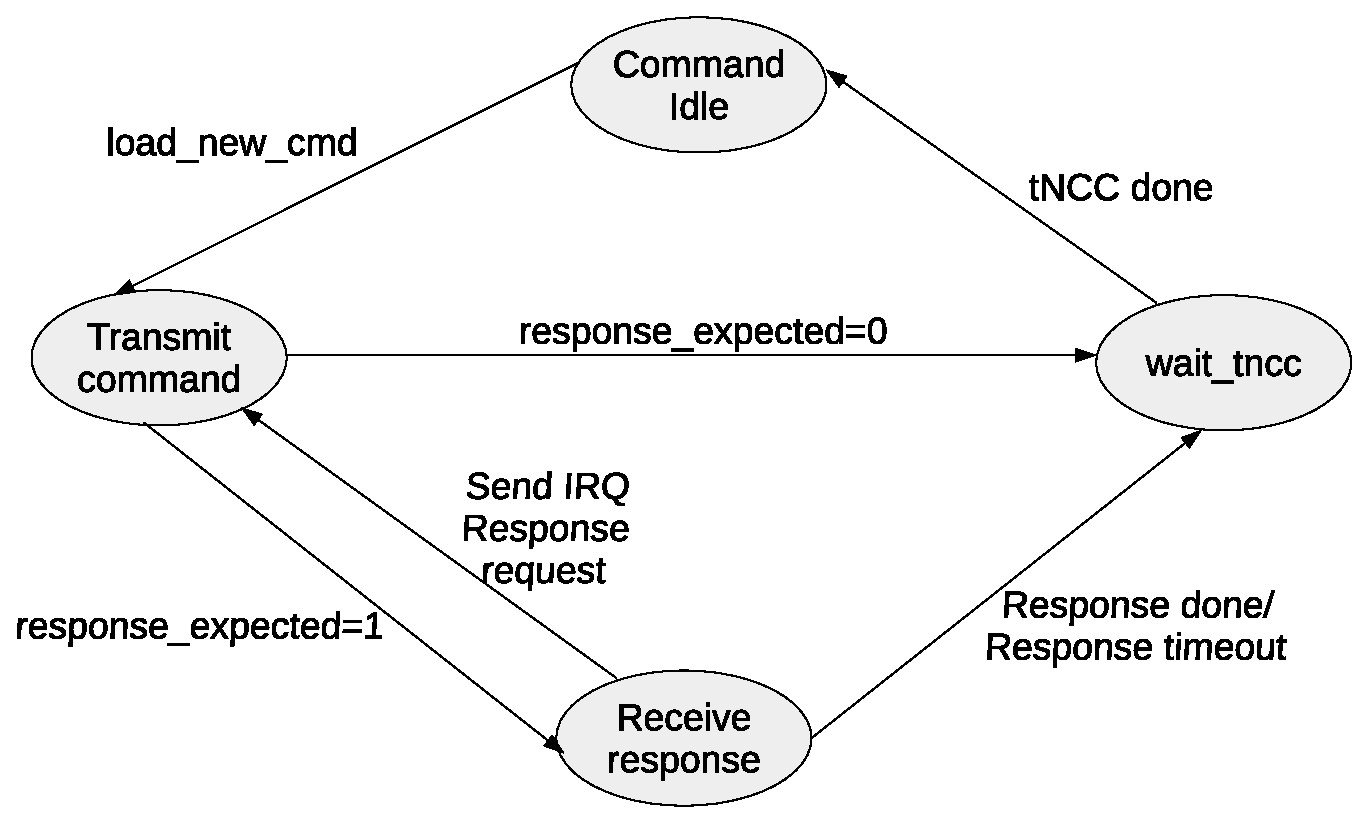
\includegraphics[width=0.55\textwidth]{./18-SDHOST/figures/18-SDHOST-cmd-state-machine.eps}
    \caption{命令通路状态机}
    \label{fig:sdhost-cmd-state-machine}
\end{figure}

\subsection{数据通路}

发送时，数据通路模块会取出 RAM 中的数据，并将其发送至 sdhost\_cdata\_out；接收时，数据通路会接收 sdhost\_cdata\_in 上的数据，并将其导入 RAM 中。数据发送命令未运行时，数据通路将加载新的数据参数，即希望发送的数据、读/写数据发送、流/块发送、块大小、字节数、卡类型、超时寄存器等。

如果在命令寄存器 (\hyperref[regdesc:CMDREG]{SDHOST\_CMD\_REG}) 中置了 SDHOST\_DATA\_EXPECTED 位，则新命令为数据传输命令，数据通路将执行以下操作之一：

\begin{itemize}
\item 若 SDHOST\_READ\_WRITE 位为 1，发送数据
\item 若 SDHOST\_READ\_WRITE 位为 0，接收数据
\end{itemize}

\subsubsection{数据发送}
接收到数据写入命令后，该模块将在两个时钟周期开始发送数据。即使命令通路在响应信息中检测到响应错误或循环冗余检查 (CRC) 错误，数据发送也会正常进行。但是，如果直到响应超时仍没有从卡接收到响应，则不发送数据。根据 \hyperref[regdesc:CMDREG]{SDHOST\_CMD\_REG} 寄存器中 SDHOST\_TRANSFER\_MODE 位的值，数据发送状态机将数据以流或块的形式加至卡数据总线上。数据发送状态机如图 \ref{fig:sdhost-tx-state-machine} 所示。

\begin{figure}[ht!]
    \centering
    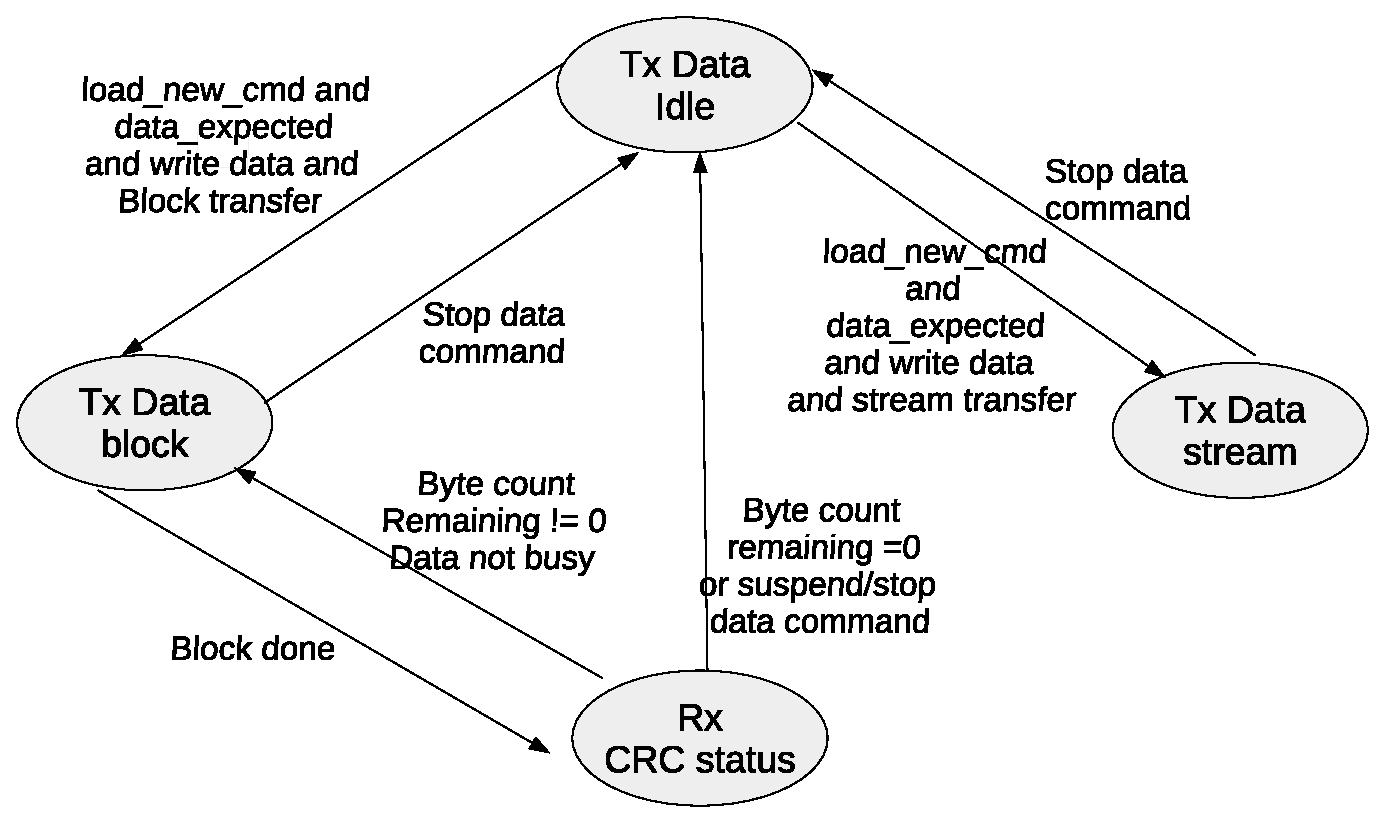
\includegraphics[width=0.55\textwidth]{./18-SDHOST/figures/18-SDHOST-tx-state-machine.eps}
    \caption{数据发送状态机}
    \label{fig:sdhost-tx-state-machine}
\end{figure}

\subsubsection{数据接收}

数据读取命令完成两个时钟周期后，该模块将开始接收数据。即使命令通路检测到响应错误或 CRC 错误，数据发送也会正常进行。如果一直未从卡接收到响应而发生了响应超时，则 BIU 无法接收到 CIU 数据发送完成的信号。如果 CIU 发送的命令是卡所禁止的非法操作，那么将无法开始读取从卡发送的数，且 BIU 也不会接收到 CIU 数据发送完成的信号。

若在数据超时前未接收到数据，数据通路将向 BIU 发出数据超时信号并结束数据传输。根据 \hyperref[regdesc:CMDREG]{SDHOST\_CMD\_REG} 寄存器中的 SDHOST\_TRANSFER\_MODE 位的值，数据接收状态机以流或块的形式从卡数据总线获取数据。数据接收状态机如图 \ref{fig:sdhost-rx-state-machine} 所示。

\begin{figure}[ht!]
    \centering
    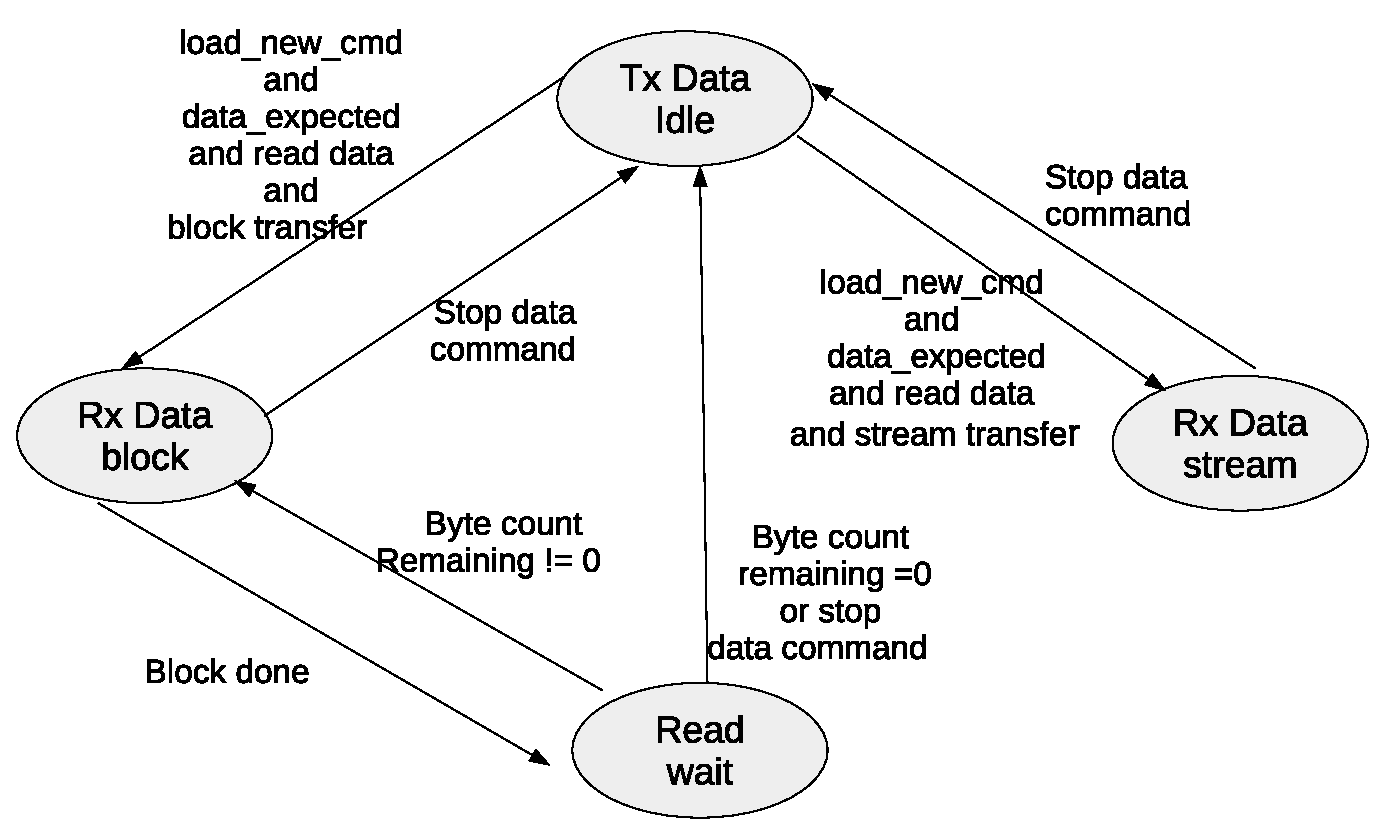
\includegraphics[width=0.55\textwidth]{./18-SDHOST/figures/18-SDHOST-rx-state-machine.eps}
    \caption{数据接收状态机}
    \label{fig:sdhost-rx-state-machine}
\end{figure}

\section{CIU 操作的软件限制}
\begin{itemize}
	\item 一次只能选择一个卡执行命令或发送数据。例如，当向某张卡发送数据或从这张卡接收数据时，不可以给另一张卡发送其它新的命令。但是，可以将新的命令发送到同一张卡上，使其读取设备状态或停止数据传输。
	\item 一次只能发出一个数据传输命令。
	\item 在开放式写卡操作期间，如果由于 RAM 为空导致卡时钟停止，那么软件必须先将数据填充到 RAM 中并启动卡时钟，然后才可以向卡发出一个停止/中止命令。
	\item 在 SDIO/Combo 卡数据传输期间，如果卡功能暂停，并且软件想要恢复所暂停的数据传输，则其必须先重置 RAM（置位 SDHOST\_FIFO\_RESET）并启动恢复命令，这和启动一个新的数据传输命令相似。
	\item 要在进行卡数据传输中发出卡复位命令（CMD0、CMD15 或 CMD52\_reset），软件必须在 \hyperref[regdesc:CMDREG]{SDHOST\_CMD\_REG} 寄存器上置位 SDHOST\_STOP\_ABORT\_CMD，保证 CIU 可以在发出卡复位命令后停止数据传输。
	\item 当在 \hyperref[regdesc:RINTSTSREG]{SDHOST\_RINTSTS\_REG} 寄存器中设置数据结束位错误时，CIU 无法控制 SDIO 中断。因此在该情况下，软件应忽略 SDIO 中断，并向卡发出停止/中止命令使其停止发送数据。
    \item 在一次读卡过程中，如果由于 RAM 已满而导致卡时钟停止，那么软件将至少读取两个 RAM 地址来重启卡时钟。
	\item 在一次命令/数据传输中只能选取一个 CE-ATA 设备。例如，当一个 CE-ATA 设备已经在传输数据，则其它 CE-ATA 设备不可传输新命令。
	\item 使能 CE-ATA 设备的中断 (nIEN=0) 后，如果该设备已经有正在执行的 SDHODT\_RW\_BLK 命令，则不可以再向这一设备发送新的 SDHODT\_RW\_BLK 命令。只有在等待 CCS 时可以发送 CCSD。
	\item 但是，如果一个 CE-ATA (nlEN=1) 设备未使能，则可以向同一设备发送新的命令来读取状态信息。
	\item CE-ATA 设备不支持开放式数据传输。
	\item CE-ATA 数据传输不支持 sdhost\_send\_auto\_stop 信号（禁止软件置位 SDHOST\_SEND\_AUTO\_STOP）。
\end{itemize}

置位命令起始位后，在发送出命令之前以下寄存器的值不可改变：

\begin{itemize}
	\item CMD --- 命令
	\item CMDARG --- 命令参数
	\item BYTCNT --- 字节计数
	\item BLKSIZ --- 块大小
	\item CLKDIV --- 时钟分频器
	\item CKLENA --- 时钟使能
	\item CLKSRC --- 时钟源
	\item TMOUT --- 超时
	\item CTYPE --- 卡类型
\end{itemize}

\section{收发数据 RAM}
RAM 子模块是一个收发数据缓冲区，分为接收和发送两个单元。也可通过 CPU 和 DMA 实现数据的收发，从而进行读写操作，可参阅章节 \ref{sec:sdhost-linked-list}。

\subsection{TX RAM 模块}
可通过两种方式使能写入操作：DMA 和 CPU 读写。

如果使能 SDIO 发送，那么可以通过 APB 接口将数据写入到 TX RAM 模块中。此时，数据将通过 APB 接口直接从 CPU 写入到 \hyperref[regdesc:BUFFIFOREG]{SDHOST\_BUFFIFO\_REG} 寄存器中。

除此之外，还可以通过 DMA 实现数据发送。

\subsection{RX RAM 模块}
可通过两种方式使能读取操作：DMA 和 CPU 读写。

当数据通路接收到数据时，该数据将被写入 RX RAM 中。可在读取端通过 APB 读取这些数据，APB 可直接读取寄存器 \hyperref[regdesc:BUFFIFOREG]{SDHOST\_BUFFIFO\_REG}。

除此之外，还可以通过 DMA 实现数据接收。

\clearpage
\section{DMA 链表环}

链表环中的每个链表模块都由两部分组成：链表和一个数据缓冲区。也就是说，每一个链表都指向一个独特的数据缓冲区，同时还连接至下一个链表模块。链表环结构如图 \ref{fig:sdhost-chain-descriptor} 所示。

\begin{figure}[ht!]
    \centering
    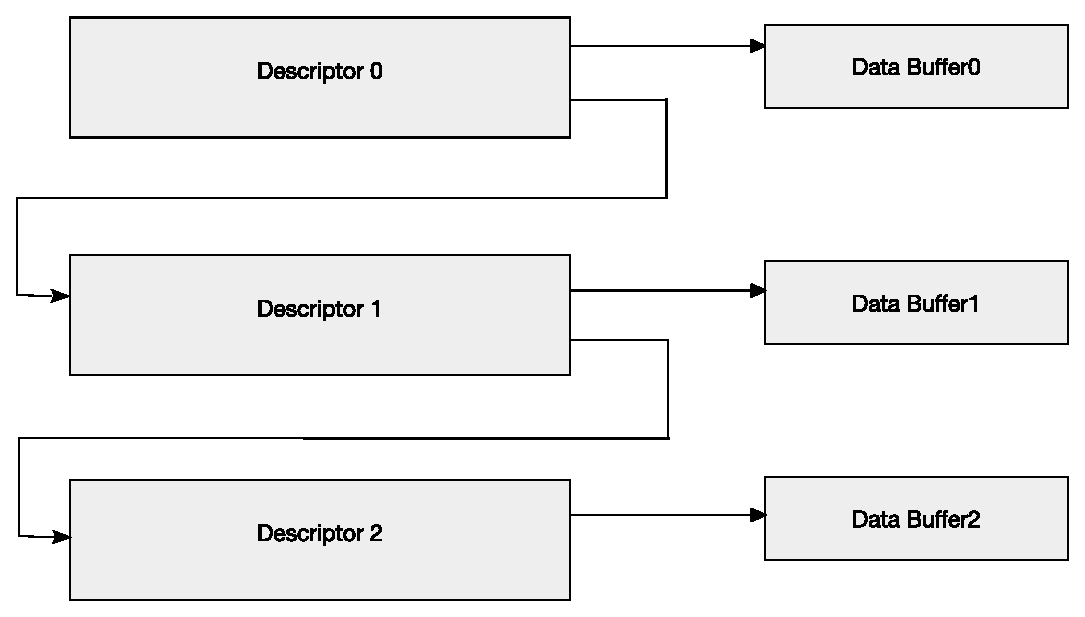
\includegraphics[width=0.6\textwidth]{./18-SDHOST/figures/18-SDHOST-chain-descriptor}
    \caption{链表环结构}
    \label{fig:sdhost-chain-descriptor}
\end{figure}

\section{DMA 链表结构}
\label{sec:sdhost-linked-list}

每个链表由 4 个字组成，如图 \ref{fig:sdhost-linked-list-structure} 所示。表 \ref{tab:sdhost-DES0}、表 \ref{tab:sdhost-DES1}、表 \ref{tab:sdhost-DES2}、表 \ref{tab:sdhost-DES3} 为这 4 个字的描述。


\begin{figure}[ht!]
    \centering
    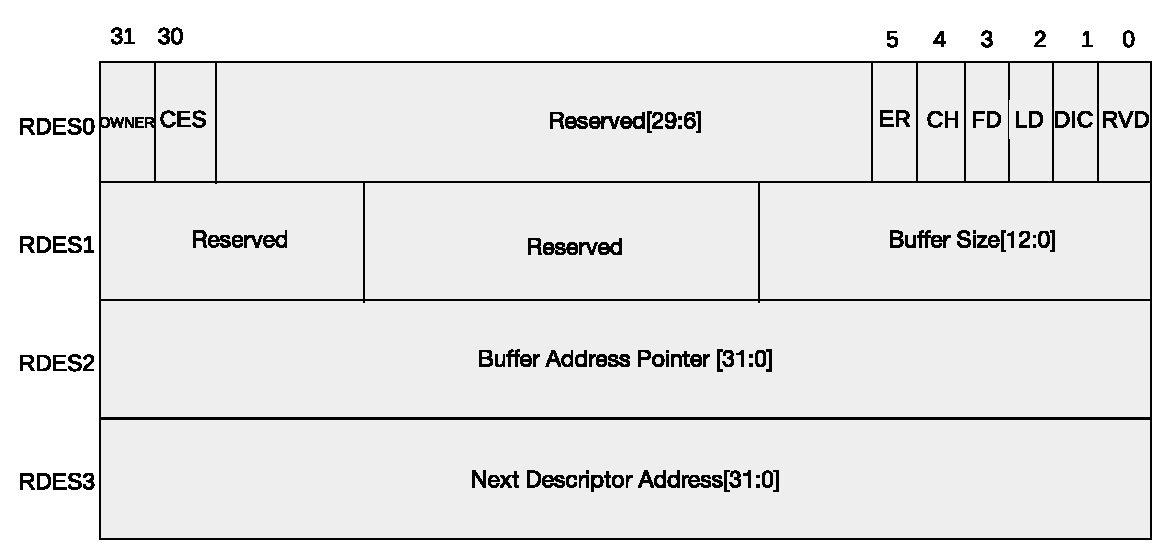
\includegraphics[width=0.7\textwidth]{18-SDHOST/figures/18-SDHOST-linkded-list}
    \caption{链表结构}
    \label{fig:sdhost-linked-list-structure}
\end{figure}

DES0 单元包含控制和状态信息。

\clearpage
\input{./18-SDHOST/tables/18-SDHOST-des0__CN}

DES1 单元包含缓冲区大小。

\input{./18-SDHOST/tables/18-SDHOST-des1__CN}

DES2 单元包含指向数据缓冲区的地址指针。

\input{./18-SDHOST/tables/18-SDHOST-des2__CN}

如果当前的描述符不是链表环中的最后一个，则 DES3 单元包含指向下一个描述符的地址指针。

\begin{longtable}[c]{ |p{3cm}|p{4cm}|p{8cm}| }
\caption{DES3 单元描述} \label{tab:sdhost-DES3}\\
\hline
\rowcolor{lightgray}
位 &名称 & 描述 \\
\hline
\endfirsthead
\hline
\rowcolor{lightgray}
位 &名称 & 描述  \\
\hline
\endhead
\endfoot
\multirow{4}{*}{31:0}& \multirow{4}{*}{\makecell[l]{Next Descriptor Address\\（下一个链表地址）}}& 如果置位 CH (DES0[4])，则该位中有指向包含下一个描述符位置的物理内存的指针。\\
&&如果该描述符不是链表环结构中的最后一个描述符，则下一个描述符的地址指针必须满足 DES3[1:0] ＝ 0。\\\hline
\end{longtable}

\section{初始化}
\subsection{DMA 控制器初始化}

DMA 控制器初始化过程如下：

\begin{enumerate}
\item 向 DMA 控制器的总线模式寄存器 (\hyperref[regdesc:BMODREG]{SDHOST\_BMOD\_REG}) 写入数据， 设置主机总线访问参数。
\item 向 DMA 控制器的中断使能寄存器 (\hyperref[regdesc:IDINTENREG]{SDHOST\_IDINTEN\_REG}) 写入数据，屏蔽不必要的中断类型。
\item 软件驱动器创建发送链表或接收链表。然后向 DMA 控制器链表基地址寄存器 (\hyperref[regdesc:DBADDRREG]{SDHOST\_DBADDR\_REG}) 中写入链表的起始地址。

\item DMA 控制器引擎尝试从链表中获取描述符。
\end{enumerate}

\subsection{DMA 控制器数据发送初始化}

DMA 控制器发送数据的过程如下：

\begin{enumerate}
\item 主机设置发送数据的描述符单元 (DES0 \verb+~+ DES3)，置位 OWNER 位 (DES0[31])，同时准备数据缓冲区。
\item 主机在 BIU 的命令 (CMD) 寄存器中写入数据命令。
\item 主机设置所需的数据发送阈值（在 \hyperref[regdesc:FIFOTHREG]{SDHOST\_FIFOTH\_REG} 寄存器中的 SDHOST\_TX\_WMARK 字段进行）。
\item DMA 控制器引擎读取描述符并检查 OWNER 位。如果 OWNER 位未置位，表明该描述符所允许的操作者为主机。此时，DMA 控制器进入挂起状态，并在 \hyperref[regdesc:IDSTSREG]{SDHOST\_IDSTS\_REG} 寄存器中产生禁能描述符中断。然后，主机需在 \hyperref[regdesc:PLDMNDREG]{SDHOST\_PLDMND\_REG} 中写入任意值来释放 DMA 控制器资源。
\item DMA 控制器等待 DHOST\_RINTSTS\_REG 寄存器中的命令完成 (CD) 位，如果 BIU 无报错，则表明数据发送已完成。
\item 然后，DMA 控制器引擎等待 BIU 发送的 DMA 总线请求，该请求将基于配置的数据发送阈值生成。对于使用突发传输不能访问的最后一个字节，则在 AHB 总线上执行单次发送。
\item DMA 控制器从主机存储器的数据缓冲区获取发送数据，并通过 RAM 将其发送至卡中。
\item 当数据跨越多个描述符时，DMA 控制器将获取下一个描述符，并继续使用后面的描述符进行后续操作。最后一个描述符位将显示该数据是否跨越多个描述符。
\item 当数据发送完成且 SDHOST\_IDSTS\_TI 位已使能，将通过置位 SDHOST\_IDSTS\_TI 将状态信息更新至寄存器 \hyperref[regdesc:IDSTSREG]{SDHOST\_IDSTS\_REG}。同时，DMA 控制器将通过对 DES0 执行写操作来清除 OWNER 位。
\end{enumerate}

\subsection{DMA 控制器数据接收初始化}

DMA 控制器接收数据的过程如下：

\begin{enumerate}
\item 主机设置接收数据的描述符单元 (DES0 \verb+~+ DES3)，置位 OWNER 位 (DES0[31])。
\item 主机在 BIU 的命令寄存器中写入读数据命令。
\item 主机设置所需的数据接收阈值（在 \hyperref[regdesc:FIFOTHREG]{SDHOST\_FIFOTH\_REG} 寄存器中的 SDHOST\_RX\_WMARK 字段进行）。
\item DMA 控制器引擎读取描述符并检查 OWNER 位。如果 OWNER 位未置位，表明该描述符所允许的操作者为主机。此时，DMA 控制器进入挂起状态，并在 \hyperref[regdesc:IDSTSREG]{SDHOST\_IDSTS\_REG} 寄存器中产生禁能描述符中断。然后，软件需在 \hyperref[regdesc:PLDMNDREG]{SDHOST\_PLDMND\_REG} 中写入任意值释放 DMA 控制器资源。
\item DMA 控制器等待命令完成位 (CD)，如果 BIU 无报错，则表明数据接收已完成。
\item DMA 控制器引擎等待 BIU 发送的 DMA 总线请求。该请求将基于配置的数据接收阈值生成。对于使用突发传输不能访问的最后一个字节，则在 AHB 总线上执行单次传输。
\item DMA 控制器从 RAM 获取数据，并将其发送至主机存储器。
\item 当数据跨越多个描述符时，DMA 控制器将获取下一个描述符，并继续使用后面的描述符进行后续操作。最后一个描述符位将显示该数据是否跨越多个描述符。
\item 当数据接收完成且 SDHOST\_IDSTS\_RI 位已使能，将通过置位 SDHOST\_IDSTS\_RI 将状态信息更新至寄存器 \hyperref[regdesc:IDSTSREG]{SDHOST\_IDSTS\_REG}。同时，DMA 控制器将通过对 DES0 执行写操作来清除 OWNER 位。
\end{enumerate}

\section{时钟相位选择}
\label{sec:sdhost-phase-selection}

如果输入数据信号或输出数据信号的建立时间的时序不符合要求，用户可以参照下图 \ref{fig:sdhost-clk-phase-selec} 改变时钟相位。

\clearpage

\begin{figure}[ht!]
    \centering
    \fbox{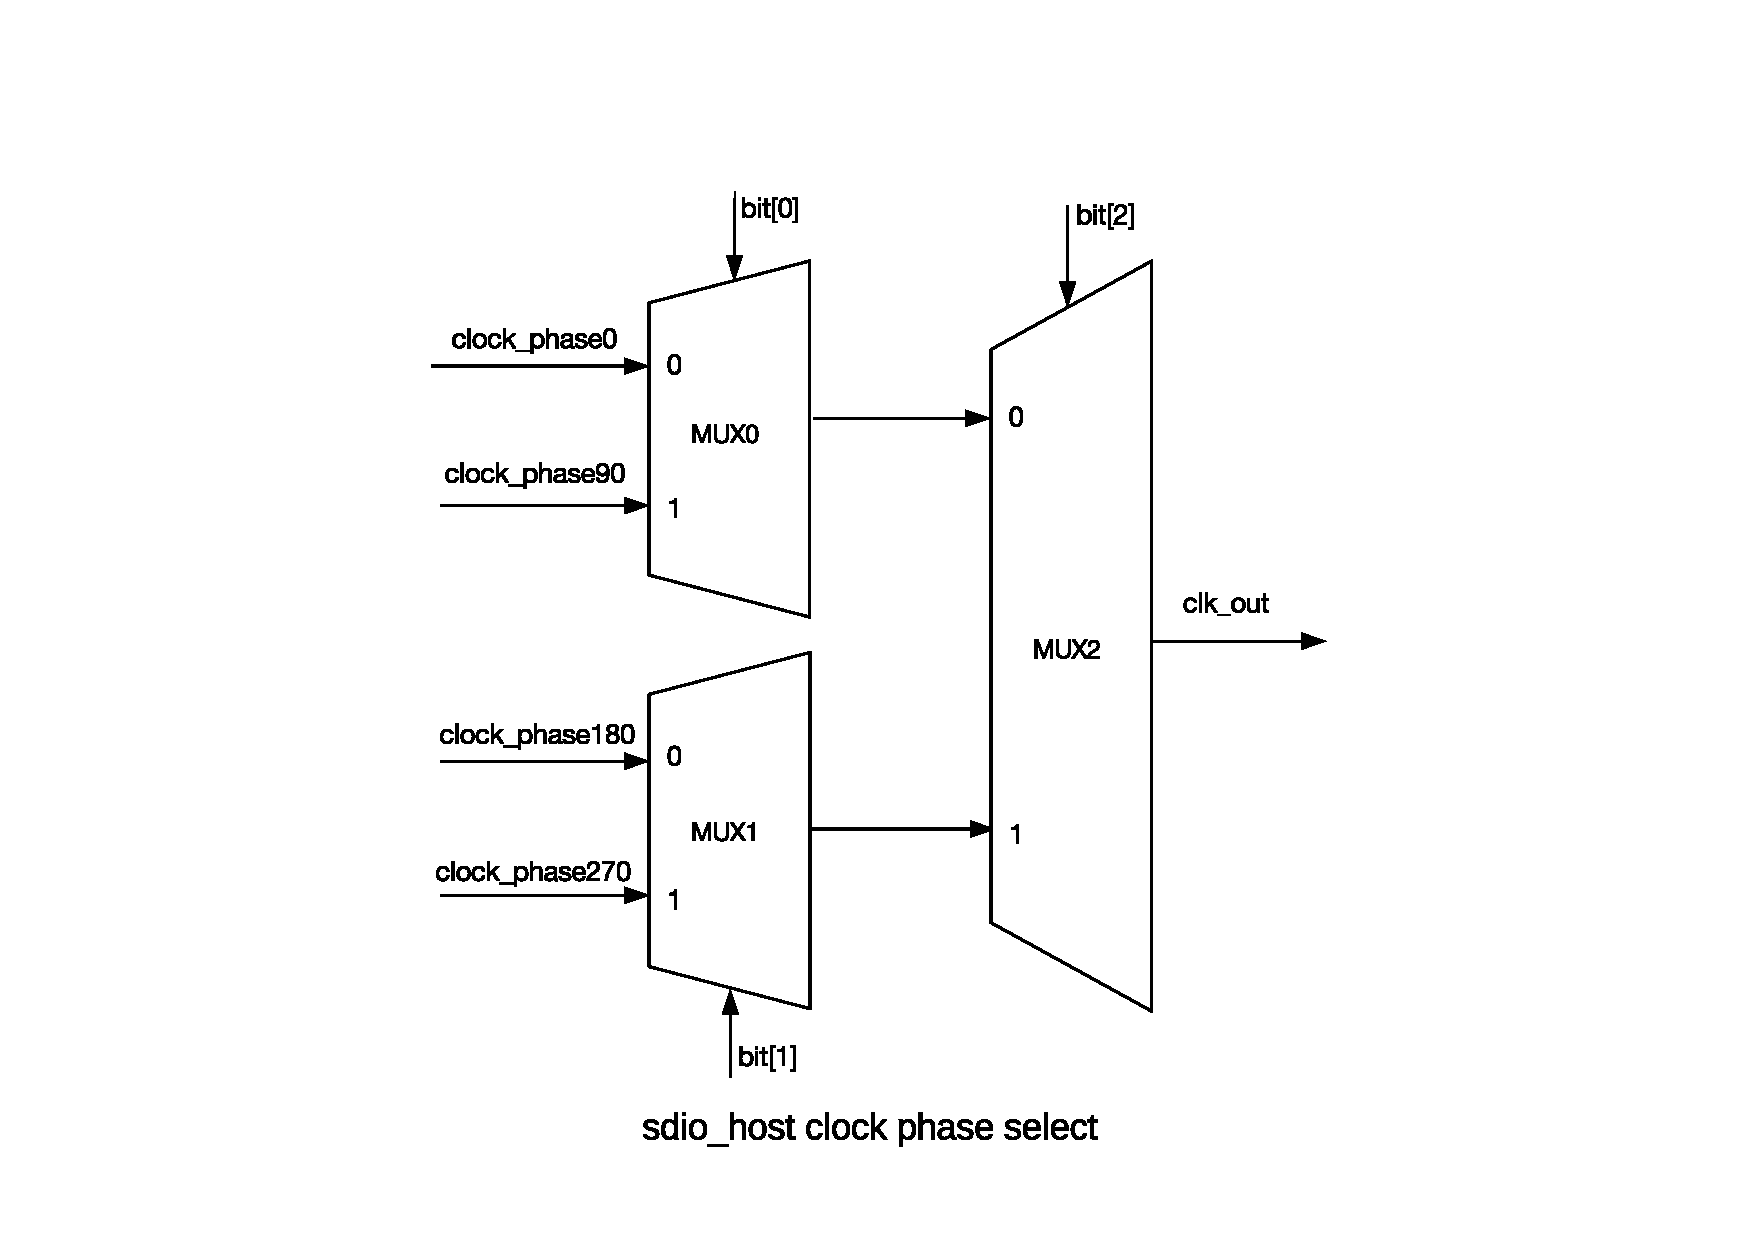
\includegraphics[width=0.5\textwidth]{./18-SDHOST/figures/18-SDHOST-clock-phase-selection.pdf}}
    \caption{时钟相位选择}
    \label{fig:sdhost-clk-phase-selec}
\end{figure}

可通过设置寄存器 \hyperref[regdesc:CLKEDGESEL]{SDHOST\_CLK\_DIV\_EDGE\_REG} 来解决时序问题。例如，清除 CCLKIN\_EDGE\_DRV\_SEL 位发送相位 0 中的输出数据，然后置位 CCLKIN\_EDGE\_SAM\_SEL 选择 90 度相位采样 SDIO 从机中的数据。如果此时仍有时序问题，还可通过向 CCLKIN\_EDGE\_SAM\_SEL 写入 4 或 6 分别选择 180 度或 270 度相位对 SDIO 从机进行数据采样。

有关时钟相位选择寄存器 \hyperref[regdesc:CLKEDGESEL]{SDHOST\_CLK\_DIV\_EDGE\_REG} 的说明，请见寄存器章节 \ref{sec:sdhost-reg}。

\input{./18-SDHOST/tables/18-SDHOST-clksel__CN}

\section{中断}
中断可在多个事件中产生。\hyperref[regdesc:IDSTSREG]{SDHOST\_IDSTS\_REG} 寄存器中包含所有可能导致中断的位。\hyperref[regdesc:IDINTENREG]{SDHOST\_IDINTEN\_REG} 寄存器中包含所有可导致中断的事件的使能位。

\hyperref[regdesc:IDSTSREG]{SDHOST\_IDSTS\_REG} 寄存器中有两组中断汇总：正常中断汇总 (第 8 位：SDHOST\_IDSTS\_NIS) 和异常中断汇总 (第 9 位：SDHOST\_IDSTS\_AIS)。置位相应的位，可以清除中断。当某组中的所有使能中断都被清除，相应的汇总位将被清零。当两组的汇总位都被清零，连接 CPU 的中断信号将撤销（停止发送信号）。

中断不排序，如果中断在驱动程序响应之前发生，则不会产生其他中断。 例如，SDHOST\_IDSTS\_RI 表示一个或多个数据已发送至主机缓冲区。

并发事件只会产生一个中断。驱动程序须扫描 \hyperref[regdesc:IDSTSREG]{SDHOST\_IDSTS\_REG} 寄存器来查找导致中断的原因。



% >>> If your module has no registers, delete sample text
%       for Sections Register Summary and Registers below <<<

%%%%%%%%%%%%%%%%%%%%%%%%
%%% Register Summary %%%
%%%%%%%%%%%%%%%%%%%%%%%%

% >>> Update the sample text below and insert
%     the info on register summary into the subfile <<<

\clearpage
\hypertarget{sdhost-reg-summ}{}
\section{寄存器列表}
\label{sec:sdhost-reg-summ}

本小节的所有地址均为相对于 SD/MMC Host Controller 基地址的地址偏移量（相对地址），具体基地址请见章节 \ref{mod:sysmem} \textit{\nameref{mod:sysmem}} 中的表 \ref{tab:sysmem-base-address}。

请查看章节 \hyperref[glossary-access-types]{\textit{寄存器的访问类型}}，了解“访问”列缩写的含义。

\subfile{\modulefiles/18-SDHOST-reg-summ__CN}


%%%%%%%%%%%%%%%%%
%%% Registers %%%
%%%%%%%%%%%%%%%%%

% >>> Update the sample text below and insert
%      the info on registers into the subfile <<<

\clearpage
\section{寄存器}
\label{sec:sdhost-reg}

本小节的所有地址均为相对于 SD/MMC Host Controller 基地址的地址偏移量（相对地址），具体基地址请见章节 \ref{mod:sysmem} \textit{\nameref{mod:sysmem}} 中的表 \ref{tab:sysmem-base-address}。

\subfile{\modulefiles/18-SDHOST-reg__CN}


\end{document}
